\documentclass[10pt]{article}
\usepackage{tmlr}
%%%%% NEW MATH DEFINITIONS %%%%%

\usepackage{amsmath,amsfonts,bm}

% Mark sections of captions for referring to divisions of figures
\newcommand{\figleft}{{\em (Left)}}
\newcommand{\figcenter}{{\em (Center)}}
\newcommand{\figright}{{\em (Right)}}
\newcommand{\figtop}{{\em (Top)}}
\newcommand{\figbottom}{{\em (Bottom)}}
\newcommand{\captiona}{{\em (a)}}
\newcommand{\captionb}{{\em (b)}}
\newcommand{\captionc}{{\em (c)}}
\newcommand{\captiond}{{\em (d)}}

% Highlight a newly defined term
\newcommand{\newterm}[1]{{\bf #1}}


% Figure reference, lower-case.
\def\figref#1{figure~\ref{#1}}
% Figure reference, capital. For start of sentence
\def\Figref#1{Figure~\ref{#1}}
\def\twofigref#1#2{figures \ref{#1} and \ref{#2}}
\def\quadfigref#1#2#3#4{figures \ref{#1}, \ref{#2}, \ref{#3} and \ref{#4}}
% Section reference, lower-case.
\def\secref#1{section~\ref{#1}}
% Section reference, capital.
\def\Secref#1{Section~\ref{#1}}
% Reference to two sections.
\def\twosecrefs#1#2{sections \ref{#1} and \ref{#2}}
% Reference to three sections.
\def\secrefs#1#2#3{sections \ref{#1}, \ref{#2} and \ref{#3}}
% Reference to an equation, lower-case.
\def\eqref#1{equation~\ref{#1}}
% Reference to an equation, upper case
\def\Eqref#1{Equation~\ref{#1}}
% A raw reference to an equation---avoid using if possible
\def\plaineqref#1{\ref{#1}}
% Reference to a chapter, lower-case.
\def\chapref#1{chapter~\ref{#1}}
% Reference to an equation, upper case.
\def\Chapref#1{Chapter~\ref{#1}}
% Reference to a range of chapters
\def\rangechapref#1#2{chapters\ref{#1}--\ref{#2}}
% Reference to an algorithm, lower-case.
\def\algref#1{algorithm~\ref{#1}}
% Reference to an algorithm, upper case.
\def\Algref#1{Algorithm~\ref{#1}}
\def\twoalgref#1#2{algorithms \ref{#1} and \ref{#2}}
\def\Twoalgref#1#2{Algorithms \ref{#1} and \ref{#2}}
% Reference to a part, lower case
\def\partref#1{part~\ref{#1}}
% Reference to a part, upper case
\def\Partref#1{Part~\ref{#1}}
\def\twopartref#1#2{parts \ref{#1} and \ref{#2}}

\def\ceil#1{\lceil #1 \rceil}
\def\floor#1{\lfloor #1 \rfloor}
\def\1{\bm{1}}
\newcommand{\train}{\mathcal{D}}
\newcommand{\valid}{\mathcal{D_{\mathrm{valid}}}}
\newcommand{\test}{\mathcal{D_{\mathrm{test}}}}

\def\eps{{\epsilon}}


% Random variables
\def\reta{{\textnormal{$\eta$}}}
\def\ra{{\textnormal{a}}}
\def\rb{{\textnormal{b}}}
\def\rc{{\textnormal{c}}}
\def\rd{{\textnormal{d}}}
\def\re{{\textnormal{e}}}
\def\rf{{\textnormal{f}}}
\def\rg{{\textnormal{g}}}
\def\rh{{\textnormal{h}}}
\def\ri{{\textnormal{i}}}
\def\rj{{\textnormal{j}}}
\def\rk{{\textnormal{k}}}
\def\rl{{\textnormal{l}}}
% rm is already a command, just don't name any random variables m
\def\rn{{\textnormal{n}}}
\def\ro{{\textnormal{o}}}
\def\rp{{\textnormal{p}}}
\def\rq{{\textnormal{q}}}
\def\rr{{\textnormal{r}}}
\def\rs{{\textnormal{s}}}
\def\rt{{\textnormal{t}}}
\def\ru{{\textnormal{u}}}
\def\rv{{\textnormal{v}}}
\def\rw{{\textnormal{w}}}
\def\rx{{\textnormal{x}}}
\def\ry{{\textnormal{y}}}
\def\rz{{\textnormal{z}}}

% Random vectors
\def\rvepsilon{{\mathbf{\epsilon}}}
\def\rvtheta{{\mathbf{\theta}}}
\def\rva{{\mathbf{a}}}
\def\rvb{{\mathbf{b}}}
\def\rvc{{\mathbf{c}}}
\def\rvd{{\mathbf{d}}}
\def\rve{{\mathbf{e}}}
\def\rvf{{\mathbf{f}}}
\def\rvg{{\mathbf{g}}}
\def\rvh{{\mathbf{h}}}
\def\rvu{{\mathbf{i}}}
\def\rvj{{\mathbf{j}}}
\def\rvk{{\mathbf{k}}}
\def\rvl{{\mathbf{l}}}
\def\rvm{{\mathbf{m}}}
\def\rvn{{\mathbf{n}}}
\def\rvo{{\mathbf{o}}}
\def\rvp{{\mathbf{p}}}
\def\rvq{{\mathbf{q}}}
\def\rvr{{\mathbf{r}}}
\def\rvs{{\mathbf{s}}}
\def\rvt{{\mathbf{t}}}
\def\rvu{{\mathbf{u}}}
\def\rvv{{\mathbf{v}}}
\def\rvw{{\mathbf{w}}}
\def\rvx{{\mathbf{x}}}
\def\rvy{{\mathbf{y}}}
\def\rvz{{\mathbf{z}}}

% Elements of random vectors
\def\erva{{\textnormal{a}}}
\def\ervb{{\textnormal{b}}}
\def\ervc{{\textnormal{c}}}
\def\ervd{{\textnormal{d}}}
\def\erve{{\textnormal{e}}}
\def\ervf{{\textnormal{f}}}
\def\ervg{{\textnormal{g}}}
\def\ervh{{\textnormal{h}}}
\def\ervi{{\textnormal{i}}}
\def\ervj{{\textnormal{j}}}
\def\ervk{{\textnormal{k}}}
\def\ervl{{\textnormal{l}}}
\def\ervm{{\textnormal{m}}}
\def\ervn{{\textnormal{n}}}
\def\ervo{{\textnormal{o}}}
\def\ervp{{\textnormal{p}}}
\def\ervq{{\textnormal{q}}}
\def\ervr{{\textnormal{r}}}
\def\ervs{{\textnormal{s}}}
\def\ervt{{\textnormal{t}}}
\def\ervu{{\textnormal{u}}}
\def\ervv{{\textnormal{v}}}
\def\ervw{{\textnormal{w}}}
\def\ervx{{\textnormal{x}}}
\def\ervy{{\textnormal{y}}}
\def\ervz{{\textnormal{z}}}

% Random matrices
\def\rmA{{\mathbf{A}}}
\def\rmB{{\mathbf{B}}}
\def\rmC{{\mathbf{C}}}
\def\rmD{{\mathbf{D}}}
\def\rmE{{\mathbf{E}}}
\def\rmF{{\mathbf{F}}}
\def\rmG{{\mathbf{G}}}
\def\rmH{{\mathbf{H}}}
\def\rmI{{\mathbf{I}}}
\def\rmJ{{\mathbf{J}}}
\def\rmK{{\mathbf{K}}}
\def\rmL{{\mathbf{L}}}
\def\rmM{{\mathbf{M}}}
\def\rmN{{\mathbf{N}}}
\def\rmO{{\mathbf{O}}}
\def\rmP{{\mathbf{P}}}
\def\rmQ{{\mathbf{Q}}}
\def\rmR{{\mathbf{R}}}
\def\rmS{{\mathbf{S}}}
\def\rmT{{\mathbf{T}}}
\def\rmU{{\mathbf{U}}}
\def\rmV{{\mathbf{V}}}
\def\rmW{{\mathbf{W}}}
\def\rmX{{\mathbf{X}}}
\def\rmY{{\mathbf{Y}}}
\def\rmZ{{\mathbf{Z}}}

% Elements of random matrices
\def\ermA{{\textnormal{A}}}
\def\ermB{{\textnormal{B}}}
\def\ermC{{\textnormal{C}}}
\def\ermD{{\textnormal{D}}}
\def\ermE{{\textnormal{E}}}
\def\ermF{{\textnormal{F}}}
\def\ermG{{\textnormal{G}}}
\def\ermH{{\textnormal{H}}}
\def\ermI{{\textnormal{I}}}
\def\ermJ{{\textnormal{J}}}
\def\ermK{{\textnormal{K}}}
\def\ermL{{\textnormal{L}}}
\def\ermM{{\textnormal{M}}}
\def\ermN{{\textnormal{N}}}
\def\ermO{{\textnormal{O}}}
\def\ermP{{\textnormal{P}}}
\def\ermQ{{\textnormal{Q}}}
\def\ermR{{\textnormal{R}}}
\def\ermS{{\textnormal{S}}}
\def\ermT{{\textnormal{T}}}
\def\ermU{{\textnormal{U}}}
\def\ermV{{\textnormal{V}}}
\def\ermW{{\textnormal{W}}}
\def\ermX{{\textnormal{X}}}
\def\ermY{{\textnormal{Y}}}
\def\ermZ{{\textnormal{Z}}}

% Vectors
\def\vzero{{\bm{0}}}
\def\vone{{\bm{1}}}
\def\vmu{{\bm{\mu}}}
\def\vtheta{{\bm{\theta}}}
\def\va{{\bm{a}}}
\def\vb{{\bm{b}}}
\def\vc{{\bm{c}}}
\def\vd{{\bm{d}}}
\def\ve{{\bm{e}}}
\def\vf{{\bm{f}}}
\def\vg{{\bm{g}}}
\def\vh{{\bm{h}}}
\def\vi{{\bm{i}}}
\def\vj{{\bm{j}}}
\def\vk{{\bm{k}}}
\def\vl{{\bm{l}}}
\def\vm{{\bm{m}}}
\def\vn{{\bm{n}}}
\def\vo{{\bm{o}}}
\def\vp{{\bm{p}}}
\def\vq{{\bm{q}}}
\def\vr{{\bm{r}}}
\def\vs{{\bm{s}}}
\def\vt{{\bm{t}}}
\def\vu{{\bm{u}}}
\def\vv{{\bm{v}}}
\def\vw{{\bm{w}}}
\def\vx{{\bm{x}}}
\def\vy{{\bm{y}}}
\def\vz{{\bm{z}}}

% Elements of vectors
\def\evalpha{{\alpha}}
\def\evbeta{{\beta}}
\def\evepsilon{{\epsilon}}
\def\evlambda{{\lambda}}
\def\evomega{{\omega}}
\def\evmu{{\mu}}
\def\evpsi{{\psi}}
\def\evsigma{{\sigma}}
\def\evtheta{{\theta}}
\def\eva{{a}}
\def\evb{{b}}
\def\evc{{c}}
\def\evd{{d}}
\def\eve{{e}}
\def\evf{{f}}
\def\evg{{g}}
\def\evh{{h}}
\def\evi{{i}}
\def\evj{{j}}
\def\evk{{k}}
\def\evl{{l}}
\def\evm{{m}}
\def\evn{{n}}
\def\evo{{o}}
\def\evp{{p}}
\def\evq{{q}}
\def\evr{{r}}
\def\evs{{s}}
\def\evt{{t}}
\def\evu{{u}}
\def\evv{{v}}
\def\evw{{w}}
\def\evx{{x}}
\def\evy{{y}}
\def\evz{{z}}

% Matrix
\def\mA{{\bm{A}}}
\def\mB{{\bm{B}}}
\def\mC{{\bm{C}}}
\def\mD{{\bm{D}}}
\def\mE{{\bm{E}}}
\def\mF{{\bm{F}}}
\def\mG{{\bm{G}}}
\def\mH{{\bm{H}}}
\def\mI{{\bm{I}}}
\def\mJ{{\bm{J}}}
\def\mK{{\bm{K}}}
\def\mL{{\bm{L}}}
\def\mM{{\bm{M}}}
\def\mN{{\bm{N}}}
\def\mO{{\bm{O}}}
\def\mP{{\bm{P}}}
\def\mQ{{\bm{Q}}}
\def\mR{{\bm{R}}}
\def\mS{{\bm{S}}}
\def\mT{{\bm{T}}}
\def\mU{{\bm{U}}}
\def\mV{{\bm{V}}}
\def\mW{{\bm{W}}}
\def\mX{{\bm{X}}}
\def\mY{{\bm{Y}}}
\def\mZ{{\bm{Z}}}
\def\mBeta{{\bm{\beta}}}
\def\mPhi{{\bm{\Phi}}}
\def\mLambda{{\bm{\Lambda}}}
\def\mSigma{{\bm{\Sigma}}}

% Tensor
\DeclareMathAlphabet{\mathsfit}{\encodingdefault}{\sfdefault}{m}{sl}
\SetMathAlphabet{\mathsfit}{bold}{\encodingdefault}{\sfdefault}{bx}{n}
\newcommand{\tens}[1]{\bm{\mathsfit{#1}}}
\def\tA{{\tens{A}}}
\def\tB{{\tens{B}}}
\def\tC{{\tens{C}}}
\def\tD{{\tens{D}}}
\def\tE{{\tens{E}}}
\def\tF{{\tens{F}}}
\def\tG{{\tens{G}}}
\def\tH{{\tens{H}}}
\def\tI{{\tens{I}}}
\def\tJ{{\tens{J}}}
\def\tK{{\tens{K}}}
\def\tL{{\tens{L}}}
\def\tM{{\tens{M}}}
\def\tN{{\tens{N}}}
\def\tO{{\tens{O}}}
\def\tP{{\tens{P}}}
\def\tQ{{\tens{Q}}}
\def\tR{{\tens{R}}}
\def\tS{{\tens{S}}}
\def\tT{{\tens{T}}}
\def\tU{{\tens{U}}}
\def\tV{{\tens{V}}}
\def\tW{{\tens{W}}}
\def\tX{{\tens{X}}}
\def\tY{{\tens{Y}}}
\def\tZ{{\tens{Z}}}


% Graph
\def\gA{{\mathcal{A}}}
\def\gB{{\mathcal{B}}}
\def\gC{{\mathcal{C}}}
\def\gD{{\mathcal{D}}}
\def\gE{{\mathcal{E}}}
\def\gF{{\mathcal{F}}}
\def\gG{{\mathcal{G}}}
\def\gH{{\mathcal{H}}}
\def\gI{{\mathcal{I}}}
\def\gJ{{\mathcal{J}}}
\def\gK{{\mathcal{K}}}
\def\gL{{\mathcal{L}}}
\def\gM{{\mathcal{M}}}
\def\gN{{\mathcal{N}}}
\def\gO{{\mathcal{O}}}
\def\gP{{\mathcal{P}}}
\def\gQ{{\mathcal{Q}}}
\def\gR{{\mathcal{R}}}
\def\gS{{\mathcal{S}}}
\def\gT{{\mathcal{T}}}
\def\gU{{\mathcal{U}}}
\def\gV{{\mathcal{V}}}
\def\gW{{\mathcal{W}}}
\def\gX{{\mathcal{X}}}
\def\gY{{\mathcal{Y}}}
\def\gZ{{\mathcal{Z}}}

% Sets
\def\sA{{\mathbb{A}}}
\def\sB{{\mathbb{B}}}
\def\sC{{\mathbb{C}}}
\def\sD{{\mathbb{D}}}
% Don't use a set called E, because this would be the same as our symbol
% for expectation.
\def\sF{{\mathbb{F}}}
\def\sG{{\mathbb{G}}}
\def\sH{{\mathbb{H}}}
\def\sI{{\mathbb{I}}}
\def\sJ{{\mathbb{J}}}
\def\sK{{\mathbb{K}}}
\def\sL{{\mathbb{L}}}
\def\sM{{\mathbb{M}}}
\def\sN{{\mathbb{N}}}
\def\sO{{\mathbb{O}}}
\def\sP{{\mathbb{P}}}
\def\sQ{{\mathbb{Q}}}
\def\sR{{\mathbb{R}}}
\def\sS{{\mathbb{S}}}
\def\sT{{\mathbb{T}}}
\def\sU{{\mathbb{U}}}
\def\sV{{\mathbb{V}}}
\def\sW{{\mathbb{W}}}
\def\sX{{\mathbb{X}}}
\def\sY{{\mathbb{Y}}}
\def\sZ{{\mathbb{Z}}}

% Entries of a matrix
\def\emLambda{{\Lambda}}
\def\emA{{A}}
\def\emB{{B}}
\def\emC{{C}}
\def\emD{{D}}
\def\emE{{E}}
\def\emF{{F}}
\def\emG{{G}}
\def\emH{{H}}
\def\emI{{I}}
\def\emJ{{J}}
\def\emK{{K}}
\def\emL{{L}}
\def\emM{{M}}
\def\emN{{N}}
\def\emO{{O}}
\def\emP{{P}}
\def\emQ{{Q}}
\def\emR{{R}}
\def\emS{{S}}
\def\emT{{T}}
\def\emU{{U}}
\def\emV{{V}}
\def\emW{{W}}
\def\emX{{X}}
\def\emY{{Y}}
\def\emZ{{Z}}
\def\emSigma{{\Sigma}}

% entries of a tensor
% Same font as tensor, without \bm wrapper
\newcommand{\etens}[1]{\mathsfit{#1}}
\def\etLambda{{\etens{\Lambda}}}
\def\etA{{\etens{A}}}
\def\etB{{\etens{B}}}
\def\etC{{\etens{C}}}
\def\etD{{\etens{D}}}
\def\etE{{\etens{E}}}
\def\etF{{\etens{F}}}
\def\etG{{\etens{G}}}
\def\etH{{\etens{H}}}
\def\etI{{\etens{I}}}
\def\etJ{{\etens{J}}}
\def\etK{{\etens{K}}}
\def\etL{{\etens{L}}}
\def\etM{{\etens{M}}}
\def\etN{{\etens{N}}}
\def\etO{{\etens{O}}}
\def\etP{{\etens{P}}}
\def\etQ{{\etens{Q}}}
\def\etR{{\etens{R}}}
\def\etS{{\etens{S}}}
\def\etT{{\etens{T}}}
\def\etU{{\etens{U}}}
\def\etV{{\etens{V}}}
\def\etW{{\etens{W}}}
\def\etX{{\etens{X}}}
\def\etY{{\etens{Y}}}
\def\etZ{{\etens{Z}}}

% The true underlying data generating distribution
\newcommand{\pdata}{p_{\rm{data}}}
% The empirical distribution defined by the training set
\newcommand{\ptrain}{\hat{p}_{\rm{data}}}
\newcommand{\Ptrain}{\hat{P}_{\rm{data}}}
% The model distribution
\newcommand{\pmodel}{p_{\rm{model}}}
\newcommand{\Pmodel}{P_{\rm{model}}}
\newcommand{\ptildemodel}{\tilde{p}_{\rm{model}}}
% Stochastic autoencoder distributions
\newcommand{\pencode}{p_{\rm{encoder}}}
\newcommand{\pdecode}{p_{\rm{decoder}}}
\newcommand{\precons}{p_{\rm{reconstruct}}}

\newcommand{\laplace}{\mathrm{Laplace}} % Laplace distribution

\newcommand{\E}{\mathbb{E}}
\newcommand{\Ls}{\mathcal{L}}
\newcommand{\R}{\mathbb{R}}
\newcommand{\emp}{\tilde{p}}
\newcommand{\lr}{\alpha}
\newcommand{\reg}{\lambda}
\newcommand{\rect}{\mathrm{rectifier}}
\newcommand{\softmax}{\mathrm{softmax}}
\newcommand{\sigmoid}{\sigma}
\newcommand{\softplus}{\zeta}
\newcommand{\KL}{D_{\mathrm{KL}}}
\newcommand{\Var}{\mathrm{Var}}
\newcommand{\standarderror}{\mathrm{SE}}
\newcommand{\Cov}{\mathrm{Cov}}
% Wolfram Mathworld says $L^2$ is for function spaces and $\ell^2$ is for vectors
% But then they seem to use $L^2$ for vectors throughout the site, and so does
% wikipedia.
\newcommand{\normlzero}{L^0}
\newcommand{\normlone}{L^1}
\newcommand{\normltwo}{L^2}
\newcommand{\normlp}{L^p}
\newcommand{\normmax}{L^\infty}

\newcommand{\parents}{Pa} % See usage in notation.tex. Chosen to match Daphne's book.

\DeclareMathOperator*{\argmax}{arg\,max}
\DeclareMathOperator*{\argmin}{arg\,min}

\DeclareMathOperator{\sign}{sign}
\DeclareMathOperator{\Tr}{Tr}
\let\ab\allowbreak

\usepackage{hyperref}
\usepackage{url}
\usepackage{graphicx}
\usepackage{booktabs}
\usepackage{longtable}
\usepackage{amsmath}
\usepackage[T1]{fontenc}
\usepackage[utf8]{inputenc}
\usepackage{microtype}
\hypersetup{colorlinks=true,linkcolor=black,citecolor=black,urlcolor=blue}

\title{Partial labels hide compositional difficulty in hand-motion data}

\author{\name Anonymous authors \email anonymous@example.org \\ \addr Paper under double-blind review}
\def\month{MM}
\def\year{YYYY}
\def\openreview{\url{https://openreview.net/forum?id=XXXX}}

\begin{document}
\maketitle

\begin{abstract}
Compositional generalisation is usually tested by holding out label combinations: a model sees every action and every tool in training, but not some of their pairings, and is scored on those. Unfortunately, the labels of hand-motion datasets were written for other purposes, and a correct label often describes only part of a recording; a split on labels then removes the label but not the motion. We test this directly. A paired penalty, the share of reconstruction error that a prior removes by seeing the held-out combinations, is calibrated with a synthetic dataset whose true penalty is zero (+2.6 \% of the naive error), planted interactions and permuted label grids. On OakInk-Image, joining clips so that each label describes only the first half of a trajectory, with data volume matched, reduces the penalty from +17.0 \% to +3.9 \%, at most 2.9 points above the control. The windows the label does describe lose 82 \% of their penalty above the control (95 \% CI 65 \% to 97 \%), so the change lies mostly in the training sets. On TACO, whose labels each name one action, a penalty predicted before its data were opened appears (+10.6 \%). Partial labels therefore hide compositional difficulty, shown here by manipulation on one dataset.

\end{abstract}

\section{Introduction}

\begin{figure}[!h]
\centering
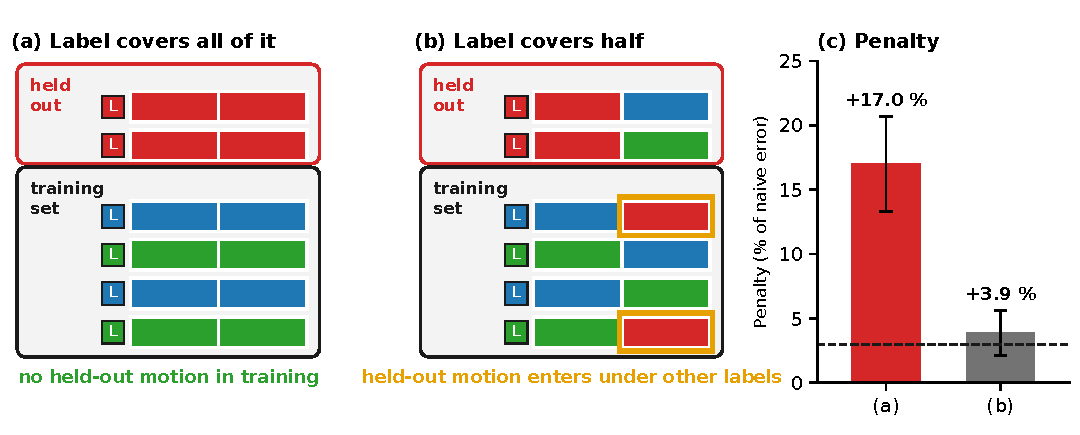
\includegraphics[width=\textwidth]{figures/fig0_teaser.pdf}
\caption{Holding out a label holds out the motion only when the label covers the whole trajectory. Each bar is a trajectory; the small square is its label and the two blocks are the motion in its two halves. Red is the held-out combination. (a) Every recording labelled red leaves training, and no red motion remains. (b) Each label covers only the first half: red motion stays in training under other labels (gold frames). (c) On OakInk-Image, with matched data volume, the penalty falls from +17.0 \% to +3.9 \%; the dashed line is the zero-truth control at the same budget (+2.96 \%). Error bars are 95 \% intervals over 40 seeds.}
\label{fig:1}
\end{figure}

Motion priors for dexterous hands learn from recorded human motion and must then produce motion that the recording does not contain. Priors with a continuous latent space \citep{yang2026lamp} and priors built from a bank of primitives are both used on the assumption that what is learned separately recombines, so that an action recorded with one tool and a tool recorded in another action remain usable together. The standard test holds out combinations of labels: every action and every tool occurs in training, some of their pairings do not, and the model is scored on those pairings. The test is established in language \citep{lake2018generalization,keysers2020measuring}, vision \citep{materzynska2020something,atzmon2020causal}, robot manipulation \citep{gao2024efficient,chen2025robohiman,wang2026diagnosing} and hand-object interaction, where TACO holds out the tool-action-object triplet while keeping every tool in training \citep{liu2024taco} and verb-noun splits with held-out objects exist for H2O and FPHA \citep{tse2025collaborative}. We adopt this design; we do not propose it.

The split is made on labels, so it holds out the motion only if each label describes the whole trajectory it is attached to. Generated benchmarks satisfy this by construction. Public hand-motion datasets need not: their annotations serve other purposes. An OakInk-Image trajectory is a single intent-oriented interaction lasting a median of 2.4 s. A TACO trajectory is described by its authors as one tool-use action and lasts a median of 4.9 s. A GRAB trajectory is a whole interaction of 8.5 s including approach and release, and an OakInk2 recording lasts a median of 20 s, with 350 of the 609 used here containing several annotated primitives. A prior trains and scores on windows of 1.07 s, so on the longer recordings a correct label describes only part of what is scored, and motion of a held-out combination enters training under another label.

A second obstacle is that the measurement has no known zero. A compositional penalty is a difference between two trained models, and two models trained on different data differ even when nothing compositional is at stake. Held-out-triplet results for hand-object motion forecasting come from one partition and one run per split \citep{liu2024taco}, so neither the size of this floor nor the spread over splits is known.

Our key insight is that the label is a proxy for the motion, and the proxy is testable. If holding out a label holds out the motion, a prior that sees the held-out combinations gains more than one that does not; if the label covers only part of each trajectory, held-out motion reaches both priors and the gain vanishes. A manipulation within one dataset tests this with everything else fixed (Figure~\ref{fig:1}), and three kinds of control tell how large a gain must be to mean anything.

Our contributions are:

\begin{enumerate}
\item A controlled demonstration that correct labels which describe only part of a trajectory reduce a compositional penalty to near the control, with most of the loss located in the training sets.
\item A calibrated protocol for held-out-combination evaluation on observational motion data, combining a zero-truth control, planted positive controls and permuted-grid controls, which shows that the floor differs between datasets.
\item A penalty declared before the data were opened and found on a fourth dataset, TACO, together with the per-seed spread of the estimate.
\end{enumerate}

Appendix D lists the sweeps on real data that the main text does not report; the per-seed results of every sweep, the gate transcripts, the written readings and a short explanatory video are supplementary material.

\section{Related work}

\textbf{Held-out combinations.} Compositional generalisation is commonly measured by withholding combinations whose parts were seen. SCAN \citep{lake2018generalization} and CFQ \citep{keysers2020measuring} do so for language, and CFQ varies how far the test distribution diverges from training across several splits; \citet{hupkes2023taxonomy} place such tests in a taxonomy of generalisation research. In vision, Something-Else holds out verb-object combinations in video \citep{materzynska2020something}. In robot learning, unseen combinations of environmental factors \citep{gao2024efficient}, of atomic skills \citep{chen2025robohiman} and of instruction components \citep{wang2026diagnosing} evaluate policies. In hand-object interaction, TACO evaluates motion forecasting on held-out triplets \citep{liu2024taco}, and \citet{tse2025collaborative} build verb-noun splits on H2O and FPHA for action recognition, removing every training sequence that contains the held-out object. These works establish the split. In generated data the label describes the trajectory by construction; where the data are recorded, as in TACO, H2O and FPHA, none of these works checks whether it does.

\textbf{When holding out a label does not hold out the target.} \citet{finegan2018improving} show that splitting text-to-SQL data by question leaves the SQL queries being predicted in both training and test, and propose splitting by query instead. SCAN contains a related case: models trained with ``turn left'' seen only as a bare command still generalise to its compositions, which the authors attribute to its output action appearing in training inside other commands, whereas they fail on ``jump'', whose action appears nowhere else \citep{lake2018generalization}. Zero-shot detection removes training images that contain unseen objects where the annotation allows it, on MS-COCO but not on Visual Genome \citep{bansal2018zero}, and zero-shot temporal activity detection removes training clips that contain an unseen activity \citep{zhang2020zstad}; both state this as protocol rather than measure what happens without it. In zero-shot action recognition, classes treated as unseen reach the training or pre-training data under other names \citep{roitberg2018towards,brattoli2020rethinking,gowda2021new}, an overlap decided class by class, by name or by visual similarity. A survey of leakage in machine-learning-based science does not single out partial label coverage among its sources \citep{kapoor2023leakage}. For motion data, a single sequence label can leave most of a motion-capture sequence undescribed: in BABEL's worked example the labelled action covers 20 \% of the sequence \citep{punnakkal2021babel}, and the temporal bounds of object interactions in egocentric video change recognition accuracy \citep{moltisanti2017trespassing}. \citet{atzmon2020causal} audit label quality on an observational compositional benchmark, and \citet{sun2023validity} show that compositional benchmarks rank the same models inconsistently, even when they share a data source. None of these measures the case in which every label is correct but describes only part of a scored trajectory; we measure it on motion data with a controlled manipulation and locate the effect in the training sets.

\textbf{Calibrating a measurement.} Each control has an origin outside compositional evaluation. A condition whose true effect is zero is the negative control of epidemiology \citep{lipsitch2010negative} and the basis of empirical calibration of estimates \citep{schuemie2014interpreting,schuemie2018empirical}; in machine learning, \citet{engstrom2020identifying} measure the bias of a replicated test set in the same spirit. Permutation nulls that preserve structure are standard for classifier evaluation \citep{ojala2010permutation}, and shuffle and random-geometry nulls calibrate cross-condition generalisation in neuroscience \citep{bernardi2020geometry}. Planting an effect of known size and measuring its recovery is the injection-recovery test of astronomy \citep{petigura2013prevalence}, the spike-in of genomics \citep{jiang2011synthetic} and, in machine learning, the planted artefact \citep{adebayo2022post}. To our knowledge they have not been combined to calibrate a held-out-combination gap.

\section{Method}

\subsection{Datasets and hand representation}

We use four public datasets: OakInk-Image \citep{yang2022oakink} (770 trajectories at 30 fps, median 72 frames), GRAB \citep{taheri2020grab} (1,048 trajectories at 30 fps, median 254 frames, from subject archives s1 to s7 and s10), OakInk2 \citep{zhan2024oakink2} (609 trajectories, motion capture subsampled by 4 to 30 fps, median 613 frames) and TACO \citep{liu2024taco} (2,317 trajectories at 30 fps, median 148 frames). Table~\ref{tab:A1} in Appendix A reconciles these counts with the published ones. OakInk-Image and OakInk2 come from the same group, so the four are not independent samples of how a hand-motion dataset can be built. Each includes MANO hand parameters \citep{romero2017embodied}. Each joint rotation is converted to Euler angles and projected onto a 27-degree-of-freedom anatomical model (four per finger, five for the thumb and six for the wrist). The flexion axis, its sign and the abduction axis are inferred from each dataset, separately for fingers and thumb, by joint-limit satisfaction, not assumed (Appendix A). Poses are normalised to [-1, 1] by the joint-limit box, so the scale is the same on every dataset.

Only the right hand is modelled. On TACO the right hand usually holds the tool \citep{liu2024taco}, so the label describes it. On OakInk-Image hand-overs, GRAB's passes and OakInk2 primitives performed by the left hand, a label can describe the other hand; this is a form of the partial coverage studied here, and it is not separated.

On OakInk-Image a trajectory's fine label is its object identity and intent; the object's category, functional class and affordance come from the dataset's own taxonomy \citep{yang2022oakink}, and for one axis the capture subject joins the fine label. On GRAB the fine label is the object and the intent verb of the sequence name; the shape class groups the 51 objects into 9 grasp-relevant classes, and the intent class groups the verbs. On OakInk2 the fine label is the recording's sequence of annotated primitives; the scene comes from the recording's metadata and the verb is the leading verb of its task sentence. On TACO the fine label is the tool-action-object triplet.

\subsection{The measuring prior}

The prior is a latent motion prior in the sense of LAMP \citep{yang2026lamp}, a Gaussian latent over a window of hand motion trained with a reconstruction term and a KL penalty; we do not propose this idea. LAMP's prior is a multilayer perceptron over an 8-step history with a 2-dimensional latent that predicts the next hand target; ours is recurrent over a 32-frame window with a 12-dimensional latent per frame, as follows. Two-layer bidirectional gated recurrent units \citep{cho2014learning} of 256 units encode a 32-frame window of 27 degrees of freedom into a 12-dimensional Gaussian latent per frame, and unidirectional ones decode it under a bounded output (2,283,059 parameters). The prior trains as a VAE \citep{kingma2014auto} whose KL weight beta \citep{higgins2017beta} rises linearly to 1.0 over the first 12 epochs, for 120 epochs on windows cut every 4 frames, with mean-squared error on pose, a first-difference term weighted 0.1 and a free-bits floor \citep{kingma2016improved} of 0.02 nats per dimension. The learning rate is 0.001 and batches hold 256 windows. The first 15 \% of each arm's training trajectories form a validation set, and the checkpoint with the lowest validation loss is scored. A window spans 1.07 s on every dataset. The prior is unconditional: it never receives a label, and labels only define the split.

The error is an autoencoding error, not a generation error. Target windows are cut every 16 frames. The encoder maps each window to the mean of its latent, and at every step the decoder receives that step's latent and the window's true first frame; it receives no other ground-truth frame. The error is the mean-squared error between output and window over all 27 normalised degrees of freedom. The penalty therefore measures how much less well a window of an unseen combination passes through the prior's bottleneck when that combination is absent from training; it does not measure whether sampling from the prior produces the combination.

\subsection{The paired compositional penalty}

A composition is one cell of a two-factor label grid, formed by grouping fine labels: on OakInk-Image, for example, the object identity is replaced by its category, functional class or affordance. On OakInk2's transitions axis a composition is instead an ordered pair of consecutive primitives within a recording's sequence.

For each seed, the protocol holds out four to six cells. The target set is about half of the trajectories in those cells, taken as whole fine labels. Two priors train on the same number of trajectories (the budget): the naive arm's training data exclude the held-out cells, and the informed arm's include the remaining trajectories of those cells, up to half its budget. Both score the same target windows. With $E_n$ and $E_i$ the naive and informed errors on the target windows, the penalty is

\begin{equation}
P = 100\,(E_n - E_i)/E_n,
\label{eq:penalty}
\end{equation}

the percentage of the naive error that the informed arm removes. Both arms share their targets, so differences in target difficulty cancel. The budget is 256 trajectories per arm unless stated. Because it counts trajectories, the training volume per arm differs between datasets (Section 4.2). Each seed draws its own split and its own random fill of both arms, and the arms share 7 \% to 42 \% of their training trajectories.

\subsection{Gates}

Four checks gate every sweep. No target's exact fine label may appear in either training set (label leak). The informed arm must reach more than 0.8 of the held-out cells with a mean of at least three trajectories per covered cell (coverage); seeds that fail are kept, and estimates without them appear where they bear on a claim. No target frame may appear verbatim in either arm's training data, checked on five seeds of each derived dataset (frame leak). For the joined-clip trajectories of Section 3.6 whose label describes every clip, no clip of a target trajectory may carry a fine label seen by either arm (constituent leak); the misaligned version fails this check by design, because its second clips carry other labels. Every split behind Section 4.2 is re-derived from its stored seed and compared with the stored record, with no mismatch in 2,144 checks.

\subsection{Controls}

\textbf{Zero-truth control.} A synthetic dataset of 3,000 trajectories at 30 fps (mean 211 frames) is built from nine grasp poses. A trajectory consists of three to seven segments between poses drawn at random, each segment following a minimum-jerk profile w(t) = 10t$^{3}$ - 15t$^{4}$ + 6t$^{5}$ as the convex combination (1 - w)a + wb of its end poses a and b; all 81 ordered pairs of poses occur. Each end pose is perturbed by a draw of scale 7$^\circ$ from a fixed six-dimensional subspace, the wrist follows its own random path, and independent noise of 0.4$^\circ$ is added to every frame before the joint coupling and limits are applied. A segment is therefore determined by its end poses up to that noise, so a pair never seen in training is reproducible from poses that were, and the true penalty is zero by construction in the data. The held-out unit is an ordered pair of poses rather than a cell of a two-factor grid, which is why the permuted grids below complement it.

\textbf{Planted controls.} A second synthetic dataset adds to each segment an offset fixed for its ordered pair and independent of its end poses, drawn at a scale of 18$^\circ$ from the same subspace and applied as sin($\pi$w), so that only trajectories containing that pair reveal it. On GRAB, a 27-dimensional offset is drawn for each shape-by-intent cell, double centring removes its additive part so that only an interaction remains, and the offset is scaled to the synthetic offset's per-frame RMS and added to every trajectory of the cell; 53 of 70 cells receive a non-zero offset. The GRAB planted sweep and its unmodified comparison use a window stride of 32.

\textbf{Permuted-grid controls.} On OakInk-Image and GRAB, the second factor is permuted over fine labels, so the number of cells, the held-out counts and the candidate cells are those of the real grid but a cell no longer groups trajectories that share their factors. TACO's action-by-tool grid is 16 \% occupied, because a tool affords few actions, and permuting one factor leaves at most 10 usable cells against 17 in 200 random draws. On TACO the cell labels are therefore shuffled over the 151 triplets, which keeps every cell's size exactly and scrambles both factors.

\subsection{Changing whether a label describes the whole trajectory}

On OakInk-Image, two clips are joined into one trajectory labelled by its first clip, with a four-frame linear cross-fade and no clip used more than once. In the aligned version both clips share their object and intent, so the label describes every window. In the misaligned version the second clip shares the object category but not the intent, so the label describes the first clip only. Both versions have 334 trajectories over the same 33 object categories, with per-category counts within one of each other, mean lengths of 204 and 200 frames, and 2,787 and 2,728 expected training windows per arm. Because 770 clips cannot supply non-overlapping trajectories at a budget of 256, both run at a budget of 64, together with the unmodified clips and the zero-truth control at that budget.

A second run on the same seeds classifies every target window as lying wholly in the first clip, wholly in the second clip or across the join, and computes the penalty within each class. If the penalty falls only because windows of other motion are scored, first-clip windows of the misaligned version keep the aligned version's penalty; if it falls because the training sets change, first-clip windows lose it as well.

\subsection{An out-of-sample prediction}

Before any TACO file was opened, we wrote down that TACO's confirmatory axis would carry a penalty above its reference, the larger of the zero-truth control and TACO's own permuted grid, together with the rule that fixes the axis: the first of action by tool, action by object and tool by object that passes the gates of Section 3.4 with coverage failing on at most 10 of 40 seeds, at the largest number of held cells from five, four and three. The rule selected action by tool with five held cells; the other two axes were not run.

\subsection{Statistics and written readings}

A seed draws a split, fills both arms and trains both priors, so each seed contributes one penalty. Two-sided Welch tests \citep{welch1947generalization} on per-seed values compare penalties, with 95 \% confidence intervals on the difference of means, against the zero-truth control at the same budget wherever one exists; the two stride-32 GRAB sweeps are compared with their unmodified sweep, and the budget-896 OakInk2 sweep with whole recordings. These tests quantify variation over seeds of one fixed dataset; comparisons between datasets compare fixed objects. Four contrasts are primary: TACO against the control, the OakInk-Image and TACO permuted grids against their real grids, and the misaligned against the aligned OakInk-Image version. All four remain below p = $10^{-5}$ after a Bonferroni correction for four tests. Held-out cells recur across seeds; refitting the four with a random effect for each held-out cell leaves all four below p = 0.002. The other tests are descriptive.

The settings and readings of the permuted-grid and planted-GRAB sweeps of Section 4.1, of every sweep in Sections 4.3 and 4.4, and of the rows of Table~\ref{tab:2} marked as such, were written down before training in documents supplied with the results. They are internal documents with file dates, not registrations time-stamped by a third party. The other rows of Table~\ref{tab:2} come from earlier sweeps of the same protocol. Seeds were never added to a sweep after its result had been seen, with one exception listed in Appendix C.

\section{Results}

\subsection{Calibration}

Table~\ref{tab:1} lists the controls. The zero-truth control returns +2.59 \% of the naive error over 20 seeds at a budget of 256 (SD 2.30) and +2.96 \% at a budget of 64 (SD 2.34, 20 seeds), both above zero. The planted synthetic control returns +9.12 \% over 18 seeds, +6.5 points above the zero-truth control (95 \% CI 4.5 to 8.6, p = 4.7 $\times$ $10^{-7}$). The planted interaction on GRAB returns +13.15 \% over 40 seeds at a stride of 32, against +0.71 \% for the same sweep without it (p = 3.1 $\times$ $10^{-9}$) and +10.6 points above the zero-truth control (p = 3.2 $\times$ $10^{-11}$). Only one size of planted interaction was run, so this shows that an interaction of that size is detected on GRAB's poses, not the smallest one that would be.

\begin{table}[t]
\caption{Calibration. Penalty as a percentage of the naive error; budget 256, window stride 4, 40 seeds unless stated. The real grid of OakInk-Image category by intent has 69 seeds.}
\label{tab:1}
\begin{center}
\scriptsize
\setlength{\tabcolsep}{3pt}
\begin{tabular}{p{0.24\textwidth}rrclcc}
\toprule
\textbf{Condition} & \shortstack{\textbf{Penalty} \\ \textbf{(\%)}} & \textbf{SD} & \shortstack{\textbf{Seeds} \\ \textbf{positive}} & \shortstack{\textbf{Compared} \\ \textbf{with}} & \shortstack{\textbf{Difference} \\ \textbf{(95 \% CI)}} & \textbf{p} \\
\midrule
Zero-truth synthetic (n = 20) & +2.59 & 2.30 & 17/20 & zero &  &  \\
Planted synthetic (n = 18) & +9.12 & 3.66 & 18/18 & zero-truth & +6.53 (4.47 to 8.58) & 4.7 $\times$ $10^{-7}$ \\
OakInk-Image category $\times$ intent, permuted & +3.65 & 6.79 & 27/40 & zero-truth & +1.07 (-1.32 to 3.45) & 0.37 \\
OakInk-Image category $\times$ intent, permuted & +3.65 & 6.79 & 27/40 & real grid & -11.53 (-14.45 to -8.62) & 5.8 $\times$ $10^{-12}$ \\
GRAB shape $\times$ fine intent, permuted & +1.38 & 6.76 & 24/40 & zero-truth & -1.21 (-3.58 to 1.17) & 0.31 \\
GRAB shape $\times$ fine intent, permuted & +1.38 & 6.76 & 24/40 & real grid & +0.06 (-2.50 to 2.62) & 0.96 \\
TACO action $\times$ tool, permuted cells & -3.39 & 6.46 & 10/40 & zero-truth & -5.97 (-8.27 to -3.68) & 2.9 $\times$ $10^{-6}$ \\
TACO action $\times$ tool, permuted cells & -3.39 & 6.46 & 10/40 & real grid & -14.01 (-17.34 to -10.69) & 2.3 $\times$ $10^{-12}$ \\
\bottomrule
\end{tabular}
\end{center}
\end{table}

The floor of the measurement depends on the dataset (Table~\ref{tab:1}, Figure~\ref{fig:2}). On OakInk-Image the permuted grid matches the synthetic control. On GRAB it equals the real grid, although its informed arm is the more exposed to held-out cells (0.38 against 0.30). On TACO it reads below the synthetic control: there the informed arm, which swaps in unrelated triplets, is worse than the naive arm (mean error 0.0303 against 0.0293). The synthetic control is therefore one reference rather than the zero of the measurement, and on TACO the declared reference, the larger of the two, is the synthetic control. The positive floor on synthetic data need not be a bias of the design alone, because a recurrent prior need not reproduce minimum-jerk interpolation exactly on pairs it has not seen; the paired design cannot separate the two. On OakInk-Image and TACO the real grids lie 11.5 and 14.0 points above their permuted grids.

\begin{figure}[t]
\centering
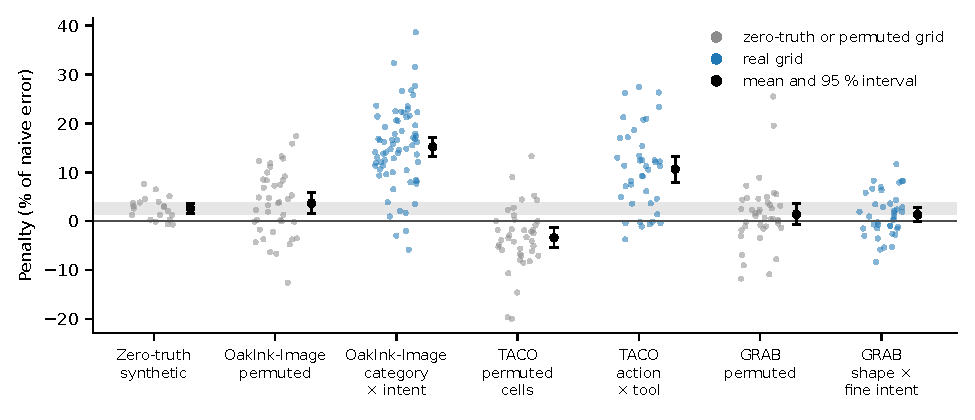
\includegraphics[width=\textwidth]{figures/fig1_per_seed.pdf}
\caption{On OakInk-Image and TACO the real label grids (blue) carry a penalty that their permuted grids (grey) do not; on GRAB neither does. Each point is one seed; black markers are means with 95 \% intervals; the grey band is the 95 \% interval of the zero-truth control's mean. Budget 256, stride 4.}
\label{fig:2}
\end{figure}

\subsection{Penalty by dataset and axis}

\begin{table}[t]
\caption{Compositional penalty by dataset and axis at a budget of 256. Windows is the expected number of training windows per arm. Held cells is the number of cells held out per seed. The 95 \% CI is of the mean over seeds. Naive error is the naive arm's mean-squared error on the target windows, the denominator of the penalty. Informed exposure is the share of the informed arm's trajectories drawn from held-out cells. p is from Welch's test against the zero-truth control. W marks rows whose settings and readings were written down before training. Rows marked $\ddagger$ are independent replications on 40 fresh seeds; the original 12-seed sweeps returned +17.9 \% (functional class by intent) and +16.7 \% (annotated transitions).}
\label{tab:2}
\begin{center}
\scriptsize
\setlength{\tabcolsep}{2pt}
\begin{tabular}{lp{0.15\textwidth}rrrrrrrrrr}
\toprule
\textbf{Dataset} & \textbf{Axis} & \textbf{Windows} & \shortstack{\textbf{Held} \\ \textbf{cells}} & \textbf{n} & \shortstack{\textbf{Penalty} \\ \textbf{(\%)}} & \textbf{SD} & \textbf{95 \% CI} & \shortstack{\textbf{Seeds} \\ \textbf{positive}} & \shortstack{\textbf{Naive} \\ \textbf{error}} & \shortstack{\textbf{Informed} \\ \textbf{exposure}} & \textbf{p} \\
\midrule
OakInk-Image & functional class $\times$ intent $\ddagger$ W & 4,591 & 4 & 40 & +22.2 & 9.4 & +19.2 to +25.2 & 39/40 & 0.0801 & 0.40 & < $10^{-12}$ \\
OakInk-Image & category $\times$ intent & 4,591 & 5 & 69 & +15.2 & 8.3 & +13.2 to +17.2 & 66/69 & 0.0672 & 0.23 & < $10^{-12}$ \\
OakInk-Image & affordance $\times$ intent & 4,591 & 5 & 130 & +12.2 & 8.2 & +10.8 to +13.6 & 124/130 & 0.0682 & 0.24 & < $10^{-12}$ \\
OakInk-Image & category $\times$ subject W & 4,591 & 4 & 40 & +10.3 & 9.0 & +7.4 to +13.2 & 37/40 & 0.0674 & 0.16 & 5.9 $\times$ $10^{-6}$ \\
TACO & action $\times$ tool W & 8,144 & 5 & 40 & +10.6 & 8.3 & +8.0 to +13.3 & 33/40 & 0.0321 & 0.46 & 6.9 $\times$ $10^{-7}$ \\
GRAB & shape $\times$ fine intent W & 17,604 & 6 & 40 & +1.3 & 4.5 & -0.1 to +2.8 & 23/40 & 0.0434 & 0.30 & 0.15 \\
GRAB & shape $\times$ intent class W & 17,604 & 5 & 40 & +2.3 & 6.2 & +0.3 to +4.2 & 29/40 & 0.0436 & 0.31 & 0.77 \\
OakInk2 & scene $\times$ verb W & 57,919 & 5 & 40 & +3.0 & 7.5 & +0.5 to +5.4 & 28/40 & 0.0166 & 0.11 & 0.78 \\
OakInk2 & scene $\times$ primitive & 57,919 & 5 & 40 & +2.3 & 7.3 & -0.0 to +4.6 & 25/40 & 0.0180 & 0.12 & 0.82 \\
OakInk2 & annotated transitions $\ddagger$ W & 57,919 & 6 & 40 & +12.2 & 10.0 & +9.0 to +15.4 & 36/40 & 0.0216 & 0.13 & 6.2 $\times$ $10^{-7}$ \\
\bottomrule
\end{tabular}
\end{center}
\end{table}

Table~\ref{tab:2} shows a penalty above the control on all four OakInk-Image axes, on TACO's axis and on OakInk2's transitions axis. The two GRAB axes and two of the three OakInk2 axes show none; on those four the 95 \% interval on the difference from the control reaches at most +3.0 points, which bounds the mean penalty above the control there. GRAB's nulls come with a planted control on the same poses (Section 4.1), so under this model, representation, metric and split its held-out shape-by-intent cells show no penalty. OakInk2 has neither a planted nor a permuted control, and its nulls are reported without interpretation. The category-by-subject axis pairs an object category with the person who grasped it; its penalty shows that the measurement responds to a held-out cell whose second factor is not an action factor, and no claim about composition rests on it.

The four datasets differ in training volume as well as in labelling, so Table~\ref{tab:2} is not a controlled comparison between datasets. OakInk-Image and TACO have the fewest training windows per arm (4,591 and 8,144, against 17,604 on GRAB and 57,919 on OakInk2), and volume moves the penalty: on OakInk2's scene-by-primitive axis the penalty is +8.56 \% at a budget of 64 against +2.30 \% at 256 (Appendix B). Volume does not act in one direction, however. On OakInk-Image a budget of 64 gives +10.15 \% against +15.19 \% at 256, a smaller penalty from less data, and OakInk2's transitions axis carries +12.2 \% at the largest volume in the table. GRAB at a budget of 64, about 4,400 windows per arm and so matched to OakInk-Image, returns +3.42 \% (SD 7.56, 40 seeds), not distinguishable from the zero-truth control at that budget (difference +0.5, 95 \% CI -2.2 to 3.1), so training volume does not account for GRAB's null. The causal evidence of this study is therefore the within-dataset manipulation of Section 4.3, where volume is matched. Appendix B adds that neither the denominator of the penalty nor the informed arm's exposure orders the datasets.

\subsection{When the label describes only part of the trajectory}

\begin{table}[t]
\caption{OakInk-Image at a budget of 64, 40 seeds each. p is from Welch's test against the zero-truth control at this budget (+2.96 \%, 20 seeds).}
\label{tab:3}
\begin{center}
\small
\setlength{\tabcolsep}{3pt}
\begin{tabular}{p{0.40\textwidth}rrcc}
\toprule
\textbf{Version} & \textbf{Penalty (\%)} & \textbf{SD} & \textbf{Seeds positive} & \textbf{p} \\
\midrule
Unmodified clips & +10.15 & 6.87 & 36/40 & 2.1 $\times$ $10^{-7}$ \\
Aligned: label describes both clips & +17.03 & 11.53 & 37/40 & 2.5 $\times$ $10^{-9}$ \\
Misaligned: label describes the first clip & +3.87 & 5.41 & 31/40 & 0.37 \\
\bottomrule
\end{tabular}
\end{center}
\end{table}

When the label describes only the first clip, the penalty is 13.2 points below the aligned version (95 \% CI 9.1 to 17.2, p = 2.1 $\times$ $10^{-8}$) and 6.3 below the unmodified clips (95 \% CI 3.5 to 9.0, p = 2.2 $\times$ $10^{-5}$), which have about 1,150 windows per arm. It lies at most 2.9 points above the control (difference +0.9, 95 \% CI -1.1 to 2.9; Table~\ref{tab:3}). Joining clips does not by itself reduce the penalty: the aligned version is above the unmodified clips (difference +6.9, 95 \% CI 2.6 to 11.1, p = 0.0019). Without the seeds that fail the coverage gate (2 aligned, 5 misaligned) the two versions read +16.46 \% and +4.89 \%, still 11.6 points apart (p = 3.5 $\times$ $10^{-7}$), with the misaligned version against the control at p = 0.056.

Misalignment changes both training sets. Averaged over ten seeds, 8.4 \% of the naive arm's training clips belong to held-out cells under another trajectory's label, so the naive arm is contaminated, and 27.9 \% of target trajectories contain a clip whose object and intent the naive arm has seen. The share of the informed arm's clips from held-out cells falls from 41.9 \% in the aligned version to 30.8 \%, so the informed arm is diluted. In the aligned version both naive-arm figures are 0 \%. In the misaligned version 61 \% of target clips belong to a held-out cell, against 100 \% in the aligned version.

\begin{table}[t]
\caption{Penalty (\%) by class of target window, same seeds and settings as Table~\ref{tab:3}; 40 seeds each. The re-run reproduced the totals of Table~\ref{tab:3} (+16.97 \% and +3.92 \%).}
\label{tab:4}
\begin{center}
\small
\setlength{\tabcolsep}{3pt}
\begin{tabular}{p{0.22\textwidth}ccc}
\toprule
\textbf{Version} & \textbf{First clip (labelled)} & \textbf{Across the join} & \textbf{Second clip} \\
\midrule
Aligned & +17.75 (SD 12.57) & +16.51 (SD 12.70) & +16.07 (SD 11.68) \\
Misaligned & +5.64 (SD 6.71) & +5.51 (SD 8.07) & +1.54 (SD 7.58) \\
\bottomrule
\end{tabular}
\end{center}
\end{table}

Table~\ref{tab:4} and Figure~\ref{fig:3} locate the loss. In the aligned version the first and second clips do not differ (paired difference +1.7, p = 0.079), so position in a joined trajectory does not matter by itself. In the misaligned version the first-clip windows, which the label describes and which show a held-out composition in both versions, read 12.1 points below the aligned version's (95 \% CI 7.6 to 16.6, p = 1.3 $\times$ $10^{-6}$), a loss of 82 \% of their penalty above the control (bootstrap 95 \% CI 65 \% to 97 \%). They remain +2.7 points above the control (95 \% CI 0.3 to 5.0, p = 0.028). The two versions consist of different trajectories, so this comparison is between different windows of the same kind and is not paired. Second-clip windows, which the label does not describe, are a further 4.1 points lower (paired p = 0.0057). Most of the loss therefore occurs on windows whose content is of the held-out kind in both versions, which locates most of it in the training sets. The design does not separate the naive arm's contamination from the informed arm's dilution; both follow from a label that describes only part of a trajectory.

\begin{figure}[t]
\centering
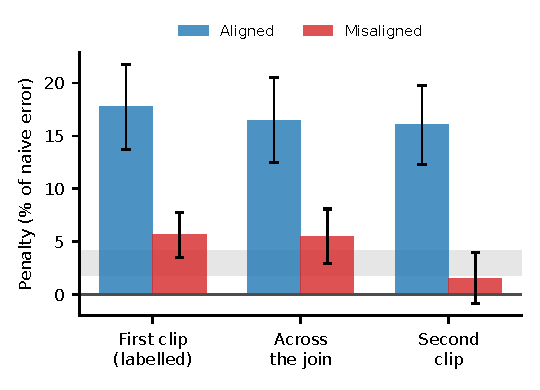
\includegraphics[width=0.62\textwidth]{figures/fig2_window_classes.pdf}
\caption{The windows the label describes lose most of their penalty in the misaligned version (red), so the change lies in the training sets rather than in the scoring. Means with 95 \% intervals over 40 seeds (Table~\ref{tab:4}); the grey band is the 95 \% interval of the zero-truth control's mean at a budget of 64.}
\label{fig:3}
\end{figure}

\subsection{The out-of-sample prediction}

TACO's trajectories last a median of 4.93 s (2.27 to 16.57 s; 1.4 \% over 10 s), and the 151 triplets of the released data combine 15 actions, 17 tools and 9 objects (the paper reports 131 triplets over 20 object categories). As predicted, its action-by-tool axis carries a penalty above the zero-truth control: +10.63 \% over 40 seeds, 8.0 points above the control (95 \% CI 5.2 to 10.9, p = 6.9 $\times$ $10^{-7}$), and +10.76 \% without the 6 seeds that fail the coverage gate. It is also 14.0 points above TACO's permuted grid (Table~\ref{tab:1}).

The per-seed estimates are widely spread. They range from -3.76 \% to +27.43 \%, with an interquartile range of +4.32 \% to +15.77 \%; 8 of 40 fall at or below the mean of the zero-truth control, and 7 exceed +20 \% (Figure~\ref{fig:2}). A seed changes the held-out cells, the random fill of both arms and the training noise together, and the design does not separate these components, so the spread is that of this paired estimate, not of the split alone.

\section{Discussion}

The split is made on labels, and the label is a proxy. On OakInk-Image, making a correct label describe only half of its trajectory, with the number of trajectories, the categories and the training volume matched, reduces a penalty of +17.0 \% to near the control. The loss occurs mostly on windows that show a held-out composition in both versions, so it lies in what the training sets contain: the rest of each trajectory carries a held-out composition into the naive arm under another label, and the informed arm's held-out trajectories are partly other motion. A penalty on TACO, whose labels each name one tool-use action, was declared before its data were seen and is found, consistent with the condition, though a positive case cannot test a necessary one.

Three points follow. First, a label that describes the whole trajectory is necessary for the penalty on OakInk-Image, but it is not sufficient for one: GRAB trajectories trimmed to their contact segment still return a penalty at the control (+2.22 \%, p = 0.78; Appendix B). Second, a paired penalty has a floor that differs between datasets. The design returns +2.6 \% when the true value is zero in synthetic data, and a permuted grid supplies a floor on each real dataset where one can be built; a test against zero would declare GRAB's shape-by-intent-class axis (+2.3 \%, p = 0.77 against the control) a compositional penalty. Third, the estimate must be read over many seeds. On TACO a single seed returns any value from -3.8 \% to +27.4 \%, so a comparison between models or splits that rests on one partition and one run cannot be read as a property of either.

These points give a short protocol for a held-out-combination split of observational motion. Check that each label describes the motion in the scored windows; where a dataset annotates action spans, report how much held-out motion enters training under other labels (Appendix B), and note that cutting OakInk2 recordings at those spans changes the penalty no more than training volume does. Hold out whole fine labels and check label, frame and constituent leaks. Report the penalty against a zero-truth control and a permuted grid on the same dataset rather than against zero. Recover a planted effect before interpreting a null. Report training volume and the distribution over many seeds.

The limitations point to future work. The error is an autoencoding error, so the results show that a prior passes an unseen composition through its bottleneck less well when it has not seen that cell, not that it cannot generate one; scoring sampled motion is the natural next test. One prior architecture is used, so the size of the penalty, though not necessarily its pattern, may differ for others. The condition is shown by manipulation on one dataset, OakInk-Image; on OakInk2 whole recordings, whose labels describe only part of each recording, a penalty still appears at a smaller training budget (Appendix B), and differences between datasets are confounded with training volume, so repeating the manipulation on a second dataset with annotated action spans would test its generality. The naive arm's contamination and the informed arm's dilution arise together, and in the misaligned trajectories the label is also less informative about intent over the whole trajectory; a design that changes one arm at a time would separate them. A permuted cell is not as compact in pose space as a real one, so an unseen composition is not separated from an unseen region of pose space; holding out pose-space clusters matched to real cells would. The aligned version exceeds the unmodified clips, possibly because a budget counted in trajectories gives the informed arm twice as many held-out clips when each trajectory holds two; this is untested.

\section{Conclusion}

Partial labels hide compositional difficulty. On OakInk-Image, a correct label that describes only part of a trajectory leaves motion of the held-out kind in the training sets, and the penalty falls to near the control; on TACO, whose labels each describe one action, a penalty declared in advance appears. On OakInk-Image, therefore, a held-out combination tests a motion model only where each label covers the whole trajectory, and whether a model appears to generalise to unseen compositions depends on how the data are labelled and on how the measurement is calibrated, as well as on the model.

\subsubsection*{Broader impact statement}

This work concerns the evaluation of motion models and has no direct application. Its main risk is the one it addresses: a compositional score read without calibration can overstate or understate what a model has learned.

\subsubsection*{Declaration of AI assistance}

A large language model was used beyond language editing: it implemented and ran the analysis scripts, launched the training runs and drafted text under author direction. The authors set the research questions, decided which claims to make and are responsible for the content. Every reported number is produced by a script operating on stored per-seed results, both supplied, so any figure can be recomputed independently of the tool.

\bibliographystyle{tmlr}
\bibliography{references}

\appendix
\renewcommand{\thetable}{A\arabic{table}}
\setcounter{table}{0}

\section{Datasets and conventions}

\begin{table}[!h]
\caption{Published and used counts.}
\label{tab:A1}
\begin{center}
\footnotesize
\setlength{\tabcolsep}{3pt}
\begin{tabular}{p{0.10\textwidth}p{0.24\textwidth}p{0.18\textwidth}p{0.30\textwidth}}
\toprule
\textbf{Dataset} & \textbf{Published} & \textbf{Used here} & \textbf{Difference} \\
\midrule
OakInk-Image & 32 object categories, 100 objects, 12 subjects (paper); 792 clips (release README) & 770 trajectories, 33 categories & clips under 40 frames are dropped; categories follow the dataset's metaV2 taxonomy file \\
GRAB & 1,334 sequences, 10 subjects, 120 Hz & 1,048 trajectories, 30 fps & the eight subject archives used here (s1 to s7, s10); subsampled by 4 \\
OakInk2 & 627 sequences (363 primitive, 264 complex task), sensors synchronised at 30 fps & 609 trajectories, 30 fps & recordings under 40 frames or without a primitive annotation are dropped; the release holds four motion-capture frames per image frame, and the frame of each image frame is kept \\
TACO & 131 triplets, 20 object categories, about 2.5K sequences & 151 triplets, 2,317 trajectories & the released data, all of which are used \\
\bottomrule
\end{tabular}
\end{center}
\end{table}

Flexion axis, flexion sign and abduction axis are inferred per dataset from joint-limit satisfaction rather than taken from documentation. On TACO this inference contradicts the dataset's own loader: without adding MANO's mean pose, 5.84 \% of values fall outside a joint limit over all 2,317 sequences, and with it 15.99 \%, so the mean pose is not added. Degrees of freedom pinned at a limit or never moving number 1 of 27 on TACO and between 1 and 6 on the other datasets; the error is computed over all 27. A held-out cell must span at least four distinct fine labels (five on GRAB's shape-by-fine-intent axis, six on OakInk2's transitions axis), and 12 to 60 cells per axis are eligible, so the spread over seeds understates the uncertainty over which cells are held. Coverage fails on 16 of 130 seeds of affordance by intent, 5 of 69 of category by intent, 6 of 40 on TACO and at most 3 of 40 elsewhere.

\section{Further experiments}

\textbf{Retargeting quality and grid density.} Clamping OakInk-Image poses so that six degrees of freedom are pinned or dead, as in GRAB, and removing whole cells of its category-by-intent grid at random to reduce occupancy from 76 \% to 49 \% (which also removed 8 categories and 243 of 770 trajectories) leave the penalty in place. The penalty was +13.70 \% and +19.64 \% respectively, against +15.19 \% unmodified (p = 0.39 and p = 0.0025).

\textbf{Stride and trimming on GRAB.} At a stride of 32 the unmodified GRAB axis does not differ from its stride-4 value in Table~\ref{tab:2} (p = 0.71). Keeping only the contact segment of each GRAB trajectory (8.5 s to 4.9 s; 58 of 1,048 trajectories dropped; about 11,400 windows per arm) gave +2.22 \%, not different from the control (p = 0.78) or from the unmodified sweep (p = 0.43).

\textbf{Denominator and exposure.} Neither the denominator of the penalty nor the informed arm's exposure orders the datasets. The naive arm's error exceeds the informed arm's by 0.0104 on OakInk-Image category by intent and by 0.0035 on TACO, against 0.0006 on GRAB shape by fine intent and 0.0004 on OakInk2 scene by primitive (means of per-seed differences). The informed arm is most exposed on TACO (0.46) and GRAB (0.30 and 0.31), which fall on opposite sides. Holding out a cell also removes part of each of its factors' data from the naive arm: averaged over held cells and both factors, the naive arm loses 31 \% to 51 \% of a held factor's trajectories on OakInk-Image, 53 \% on TACO, 30 \% to 31 \% on GRAB and 49 \% to 52 \% on OakInk2, so this loss does not order the datasets either. Within an axis it relates weakly to the per-seed penalty on OakInk-Image (r = +0.11 to +0.34) and on TACO (r = +0.25, p = 0.12).

\textbf{Contamination on OakInk2.} OakInk2 annotates the frame span of each primitive, so contamination is measurable there. On its scene-by-primitive axis the labelled primitive covers a median of 57 \% of a recording's frames, 259 of 609 recordings hold a single primitive, and over the sweep's 40 splits 11.6 \% of the naive arm's training recordings contain a held-out scene and primitive after their first primitive (4.9 \% of its training frames), while 40 \% of target frames are the held-out primitive.

\textbf{Budget on OakInk2.} Whole OakInk2 recordings on the scene-by-primitive axis returned +2.30 \% at a budget of 256 and +8.56 \% at a budget of 64 (difference +6.3, p = 0.0097; the latter above its control, p = 0.011). Recordings cut at their annotated primitive boundaries and labelled by their own primitive returned +8.93 \% at a budget of 256, which is close to the frame volume of whole recordings at 64 (68,326 against 59,806 frames per arm) and did not differ from them (p = 0.89), and +5.19 \% at a budget of 896, which matches the frame volume of whole recordings at 256 and was not above them (difference +2.9, 95 \% CI -0.5 to 6.3, p = 0.097). On OakInk2, therefore, cutting recordings changes the penalty no more than the volume of training data does, and the whole-recording null is reported without a cause.

\section{Departures from plan}

The affordance-by-intent sweep was extended from 70 to 130 seeds after its first 70 had been seen; this is the one exception to the rule of Section 3.8, and no claim rests on that axis alone. An interim value of the category-by-subject sweep was seen at 28 of 40 seeds through a scripting side effect; its seed list and readings were not changed. Window stride was not uniform in the earliest sweeps; the two affected axes were re-run at the common stride, which left the GRAB axis unchanged and turned the OakInk2 transitions axis from +3.44 \% at a stride of 16 into the penalty of Table~\ref{tab:2}. A first version of the joined OakInk-Image trajectories reused source clips, so that target frames appeared in training; it was discarded and the frame-leak gate was added. A second version joined clips of different objects under one fine label, which exposed the informed arm to the targets' objects; it was replaced by the version of Table~\ref{tab:3} and the constituent-leak gate was added. A test of whether cutting OakInk2 recordings at primitive boundaries creates a penalty was withdrawn when its declared data-volume control reproduced the effect (Appendix B). Two axes were first run at 12 seeds in an earlier phase; their replications on 40 fresh seeds were declared before they started, and Table~\ref{tab:2} reports the replications. The OakInk2 loader originally took the motion capture to run at the published 30 fps of the synchronised sensors; the release holds four motion-capture frames per image frame, so the frames kept are at 30 fps, which changes only the durations reported for OakInk2, not any penalty.

\section{Every sweep run under the protocol}

Sweeps on real data not reported in the main text, with their results (the prior of Section 3.2; penalty as a percentage of the naive error; budget 256 and stride 4 unless stated). Sweeps of a second prior architecture, run for a comparison outside the scope of this paper, and development runs on synthetic data are listed in the supplement.

{\footnotesize
\setlength{\tabcolsep}{3pt}
\begin{longtable}[c]{p{0.40\textwidth}cc p{0.32\textwidth}}
\toprule
\textbf{Sweep} & \textbf{n} & \textbf{Penalty (\%)} & \textbf{Why not in the main text} \\
\midrule
\endhead
\bottomrule
\endlastfoot
OakInk-Image category $\times$ intent, second set of models on the same 70 seeds & 70 & +14.78 & Trained for a comparison with a second architecture; agrees with Table~\ref{tab:2}, whose 69 seeds are those on which both architectures finished \\
OakInk-Image object-id prefix $\times$ intent, four sweeps & 18 to 70 & +14.30 to +17.81 & The prefix marks a sub-collection, not a category; superseded by the official taxonomy \\
OakInk-Image object $\times$ intent, budgets 256 and 64 & 5 & +5.56 and -2.22 & 2.2 trajectories per cell, too few to split \\
DexYCB subject $\times$ object, two versions & 12 & +0.09 and +1.12 & No action factor; early split code \\
GRAB shape $\times$ fine intent with contact channels, two inputs, stride 32 & 20 & -0.03 and +0.90 & Different input channels \\
GRAB shape $\times$ fine intent, first run, stride 32 & 2 & -10.12 & Stopped; replaced \\
GRAB contact segment, stride 4 & 7 & -1.35 & Stopped to free the GPU; the stride-32 sweep is in Appendix B \\
OakInk2 annotated transitions, stride 16, two versions & 12 & +9.06 and +3.44 & Stride 16 and early split code; replaced at stride 4 \\
OakInk2 primitive segments, two further sweeps & 20 and 40 & +8.97 and +7.14 & Confounded with training volume (Appendix B) \\
OakInk-Image joined clips, five earlier versions, budgets 256 and 64 & 11 to 40 & +3.03 to +57.24 & Reused clips or leaked constituents (Appendix C) \\
OakInk2 subject $\times$ verb, three held cells & - & - & Started; not completed \\
\end{longtable}}

\end{document}
